%\documentclass[letterpaper, 10 pt, conference]{ieeeconf}  % Comment this line out
                                                          % if you need a4paper
\documentclass[a4paper, 10pt]{IEEEconf}      % Use this line for a4
                                                          % paper

%\IEEEoverridecommandlockouts                              % This command is only
                                                          % needed if you want to
                                                          % use the \thanks command
%\overrideIEEEmargins
% See the \addtolength command later in the file to balance the column lengths
% on the last page of the document
\providecommand{\tabularnewline}{\\}
%% Because html converters don't know tabularnewline

% The following packages can be found on http:\\www.ctan.org
%\usepackage{graphics} % for pdf, bitmapped graphics files
%\usepackage{epsfig} % for postscript graphics files
%\usepackage{mathptmx} % assumes new font selection scheme installed
%\usepackage{times} % assumes new font selection scheme installed
%\usepackage{amsmath} % assumes amsmath package installed
%\usepackage{amssymb}  % assumes amsmath package installed
\usepackage[utf8]{inputenc}
\usepackage{amsmath}
\usepackage{float}
\usepackage[T1]{fontenc}
\usepackage{graphicx}
\usepackage{textcomp}
\usepackage{hyperref}
\graphicspath{ {images/} }


\title{\LARGE \bf The correlation between Smart-cities and gentrification }

\author{Jérémy Scheurer, Philipp Miotti and Rob Spaargaren}

\begin{document}

\maketitle
\thispagestyle{empty}
\pagestyle{empty}


%%%%%%%%%%%%%%%%%%%%%%%%%%%%%%%%%%%%%%%%%%%%%%%%%%%%%%%%%%%%%%%%%%%%%%%%%%%%%%%%
\begin{abstract}
Gentrification is the process of wealthier citizens moving into a poor neighbourhood and investments being made to increase the living quality, therefore increasing living costs and driving out the poorer inhabitants. A city which becoes "Smart", by introducing sensors, information and communication technologies to increase the quality of life, might spur an influx of wealthy citizens, causing gentrification. In this paper we have constructed a metric based on the evolution of household incomes between different city districts over a period of 2008-2016 and on the district distances, to quantify gentrification. Given a ranking of the Smartness of a city, we applied our metric to Smart and non-Smart cities to compare their gentrification. Calculating the metric for a set of 12 Smart cities and a set of 9 non-Smart cities from the same countries, gives an average of 82 $\pm$ 123 for Smart cities and 59 $\pm$ 52 for non-Smart cities. These numbers do not indicate a statistically significant difference between both sets, and therefore we cannot conclude that there is a link between gentrification and the Smartness of a city.

%Maybe mention that our contribution is also a novel dataset with distances and household incomes for international cities. 

\end{abstract}


%%%%%%%%%%%%%%%%%%%%%%%%%%%%%%%%%%%%%%%%%%%%%%%%%%%%%%%%%%%%%%%%%%%%%%%%%%%%%%%%
\section{Introduction}
\label{sec:Introduction}
The technological progress of our society shapes our daily life in an unprecedented
way and faster than ever before. Since the introduction of the internet, our world 
has become progressively more connected and new ways of collecting data are introduced
continuously. This data is used to make better decisions, provide better solutions and  implement new systems to improve the quality of life.
Following this trend, modern sensors are deployed in different areas of a city
(e.g. public transport, parking sensors, citizen participation, clean energy, smart buildings, car sharing etc. [2]) to improve the functioning of these systems 
and offer high quality services to the citizens. A city that deploys many of these systems
to improve the general quality of life of its citizens is called a Smart city.

A city which develops into a Smart city greatly increases the living standard
for its citizens, making it more attractive for people to move to this town. This might spur an 
influx of wealthy inhabitants, who also move into the poorer districts of the city,
since these districts also experience a great increase in quality of living. These new,
wealthy inhabitants and investors following this trend invest money to increase the quality of their neighbourhood even further,
leading to increasing living costs, driving out the poorer former residents. This 
process of wealthy inhabitants moving in a neighbourhood, investing money to renovate
the neighbourhood, increasing the living quality and living costs and
driving out the poorer former residents, is called gentrification. Therefore, 
there might be a link between gentrification and the development of cities becoming Smart. There are many reasons why finding this link is important. The effects of gentrification are manifold and are often very controversial. On one hand ther is usually a reduction of crime, more incentives for property owners to increase/improve housing, stabilization of declining areas, increased property values and more \cite{c5}. But on the other hand there is a displacement of inhabitants because of rent/price increases and with this a loss of affordable housing. Also there is a commercial/industrial displacement and property prices might be unsustainable in the long term. Lastly, there are effects such as community resentment and conflict, loss of social diversity and displacement and housing pressure on neighbouring areas\cite{c5}.
The importance of investigating this link lies in the possibility for cities to pre-emptively
change their policies to protect the poorer residents and prevent the neighbourhoods these
citizens move into from deteriorating.

To investigate whether this link exists, a quantity indicating the Smartness
of a city should be compared to a quantity characterizing the degree of gentrification
of the city. To give an indication of the smartness of a city, we will use two publicly
available rankings of cities across the globe. The ranking of a city across both lists
is used as an indicator of the Smartness of the city. The lists we have used are published
by the IESE Business School of the Universtiy of Navarra \cite{c1}, and by the Easypark group \cite{c2},
an international group specialising in implementation of smart parkings in cities.

Initially, gentrification was defined by Ruth Glass in 1964 as the displacement of lower-class
working residents in urban neighbourhoods by middle-class citizens \cite{gentr_def}. This definition
is not useful to quantitatively measure gentrification, so the wide effects of gentrification on a neighbourhood should be utilized.
There is a wide variety of effects of gentrification on the neighbourhood, which could be used
to quantify it. The nature of the neighbourhood changes, affecting not only housing prices and
living costs, but also the look of the neighbourhood, by increasing the amount of public green
and parks, and the number of schools. Gentrification also induces a shift in demographics, in
culture, educational level and household income. These effects have been used in both qualitative
and quantitative research (see Barton, 2016, for an overview \cite{Barton}). However, the changes
in neighbourhood characteristics could be due to a number of other factors like a change of policy
by the city government rather than gentrification, and can be subjective of nature. Of the effects
on characteristics of the population, an increase of income is the most indicative and least 
subjective sign of the transition to a higher social class. Using a quantity based on household
income to measure gentrification has also been used in other quantitative studies \cite{gentr_research}.
We present a metric based on the Gross Disposable Household Income (GDHI) that quantifies gentrification
in this paper.

%Add another paragraph! Describe data collection and why we used a data science approach.
%Add that we also look at non-Smart cities for comparison.
%Mention database on gitlab and additional importance of presenting the dataset.
%Maybe mention the paper of the stanford guys...and the paper which looked at gentrification in 7-8 american cities. 

\section{Gentrification Index as a metric}
\label{sec:Gentrification}
To quantify gentrification, we have developed a metric based on the GDHI of different districts of a city, which meets certain requirements.
Firstly, we require our metric to be independent of the initial state of a city (temporal independence),  i.e., to capture merely the
gentrification in a certain timespan irrespective of the mutual differences between city parts at an initial time from which the analysis
has started.  As we look at a time frame of 2008-2016, this has the added benefit that we can really ignore previous gentrification processes and the factors that influenced it. Also the process of becoming a Smart city is relatively new, it might represent itself in this contemporary time frame. Moreover, it should be possible to compare the extent of gentrification for various cities from all over the world (spatial independence).
Thus, we have to make it independent of the local currency and of the overall wealth of a city. In addition, a weighting shall be applied to the
neighbourhoods based on their distance. Differences between adjacent and close neighbourhoods will be weighted more heavily than differences between
those that are far apart, as the notion of gentrification tries to capture local distinctions. Lastly, we require it to be a 
non-negative, strictly increasing, and intensive quantity. The last properties imply that the index is zero, if all districts have the same GDHI, 
and it increases, if the income gap also increases. Intensiveness of our metric means that the it does not scale with the size of the city or with
the number of districts.

We propose the change of the GDHI with respect to time as our central quantity to derive our metric. The change of GDHI is compared between the different
districts of a city, where the division of a city into districts is  by virtue of administrative division units ADU. To study the temportal change of GDHI
between different districts across the same timespan, to avoid noise induced by different conditions prevalent to different times, we compared the data of
each district in the timespan 2008-2016. How the units for a particular city were actually chosen is described in section III.
To assure temporal independence, we calculate the increase of the GDHI in each ADU $x_{i}=x(District = District_i)$ relative to the increase of the GDHI 
averaged over the whole city, $\tilde{x}$. More precisely, 

\begin{equation}
\begin{split}
x_{i}=\frac{\mathrm{GDHI}(i,2016)-\mathrm{GDHI}(i,2008)}{\mathrm{GDHI}(i,2016)}, \\
\quad\tilde{x}=\frac{\widehat{\mathrm{GDHI}}(2016)-\widehat{\mathrm{GDHI}}(2008)}{\widehat{\mathrm{GDHI}}(2016)},
\end{split}
\label{eq:gdhi}
\end{equation}

where $\ \widehat{}\ $ denotes the average of GDHI in a particular year over all districts $i$. To normalize this increase of income
in district $i$ with respect to the increase of income of the rest of the city, and to make it independent of valuta and other city-specific
factors, we will use $r_{i}=\left(x_{i}-\tilde{x}\right)/\tilde{x}$ in our metric. Table \ref{tab:Median-household-income} shows this relative
increase of the GDHI in case of Berlin, which suits as an example to demonstrate our metric. Two normalizations were used in the above definitions: 
one in $x_{i}$ or rather $\tilde{x}$, and the other in $r_{i}$.
Because an absolute gentrification is not sensible, we have to choose relative variables for our gentrification measure. 
The contribution of the first is twofold; we normalize the GDHI to a specific arbitrary year. This corresponds to a temporal 
normalization. Without the second ''spatial'' normalization, we would not be able to compare the cities with each other. 

\begin{table}[h]
	\begin{centering}
		\begin{tabular}{|c|c|c|c|}
			\hline 
			District & $\mathrm{GDHI}(i,2008)$ & $\mathrm{GDHI}(i,2016)$ & $\left|r_{i}\right|$ \tabularnewline
			\hline 
			\hline 
			$1$ & $22000$ & $27900$ & $0.14$\tabularnewline
			\hline 
			$2$ & $18000$ & $21300$ & $0.37$\tabularnewline
			\hline 
			$3$ & $17700$ & $25500$ & $0.25$\tabularnewline
			\hline 
			$4$ & $19600$ & $24300$ & $0.21$\tabularnewline
			\hline  
			$5$ & $16200$ & $21900$ & $0.05$\tabularnewline
			\hline 
			$6$ & $18800$ & $23700$ & $0.16$\tabularnewline
			\hline 
			$7$ & $14800$ & $21600$ & $0.27$\tabularnewline
			\hline 
			$8$ & $17400$ & $25800$ & $0.32$\tabularnewline
			\hline 
			$9$ & $15500$ & $20400$ & $0.02$\tabularnewline
			\hline 
			$10$ & $17400$ & $21900$ & $0.17$\tabularnewline
			\hline 
			$11$ & $17700$ & $23400$ & $0.01$\tabularnewline
			\hline 
			$12$ & $17800$ & $24600$ & $0.13$\tabularnewline
			\hline 
		\end{tabular}
		\par\end{centering}
	
	\caption{Median household income per month in EUR in Berlin (city divided into
		districts according to Figure \ref{fig:map_berlin} in years
		2008 \& 2016, along with normalized increase of income $r_i$.}
		\label{tab:Median-household-income}
\end{table}


\begin{figure}
	\centering{}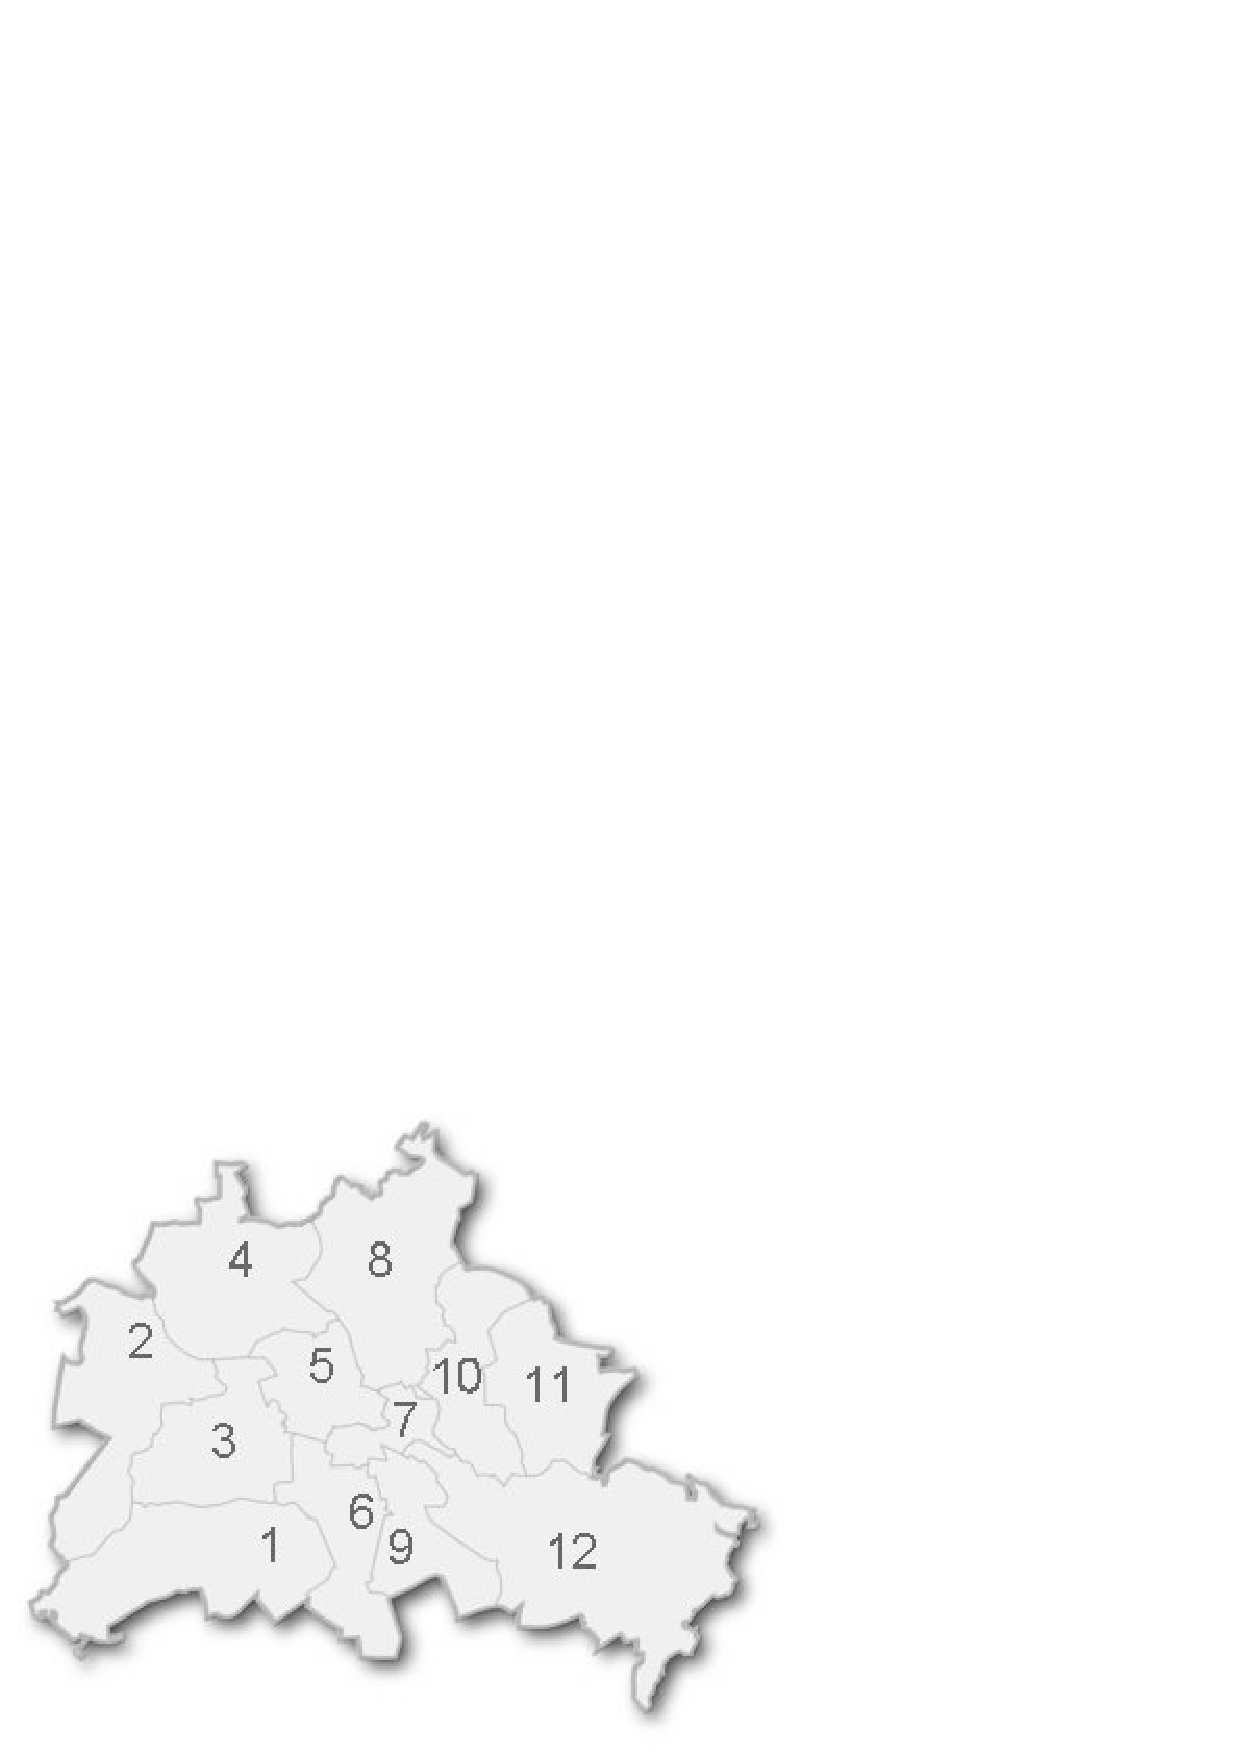
\includegraphics[scale=0.5]{stadtplan-berlin.jpg}
	\caption{Map of Berlin's districts with random numbering. Image: © Increa}
	\label{fig:map_berlin}
\end{figure}

The next step consists of defining a measure for the distance of a district with respect to each other. 
A generic solution is to use the ADU structure of a city, the districts themselves as distance units. 
Therefore, we introduce the number of minimal district-border-crossings, which are necessary to get from 
district $i$ to district $j$, as our distant measure. For example, the distance, denoted as $\left\langle \cdot,\cdot\right\rangle $,
of district 1 to district 8 in Figure \ref{fig:map_berlin} is equal to 3, i.e. $\left\langle 1,8\right\rangle =3$.
Hence, differences in the values $r_{i}$ of district further apart contribute less to the gentrification index $g_{i}$
of an particular district $i$. For the sake of intensiveness we have to normalize this distance by the total number of 
districts in a city. How the distances are calculated exactly is explained in section III.

The final step consists of putting the quantities $\left\langle \cdot,\cdot\right\rangle $ and $r_{i}$ together 
in a way which results in a meaningful formula for gentrification satisfying our requirements, 

\begin{equation}
G=\sum_{i=1}^{N}G_{i},\quad G_{i}=\frac1{N}\sum_{j=1,\,j\neq i}^{N}\frac{\left|r_{i}-r_{j}\right|^{2}}{\left\langle i,j\right\rangle },
\label{eq:gindex}
\end{equation}

Where $N$ is the number of districts in the city.
We call $G$ and $G_{i}$ the gentrification index of a city and the gentrification index of district $i$ respectively.
Due to the fact that gentrification is a rather subjective notion, and the fact that in the perspective of citizens it manifests 
itself the most when adjacent neighborhoods are compared, we take the square of our distance measure $\left\langle \cdot,\cdot\right\rangle $.
This has the effect to soften the differences between two districts when they are far apart. The meaning of the numerator in Equation \ref{eq:gindex}
is clear when we write out the squares, $\left(x_{i}^{2}-x_{j}^{2}\right)/\tilde{x}^{2}.$ The numerator is smaller, 
if the mean GDHI of the city $\tilde{x}$ is high. Then, two district with a big difference in the GDHI $x_{i}-x_{j}$ are going 
to make $G_{i}$ small, whereas on those where the difference is small $\tilde{x}$ has no effect at all. With this feature we can 
take into account the overall increase of the GDHI in a city. The gentrification index of an city with a low $\tilde{x}$ but a distinctive 
shift of citizens of different working-classes shall be especially big, as we can then assume that wealthier people haven't moved in from 
beyond the city at an above average rate.

Although, the above argumentation is sensible, we can't be sure if Equation \ref{eq:gindex} is the best formula for the index. Thus, we also present
some alternatives to $G_{i}$, and compare these to the equation. Namely, 

\begin{equation}
\begin{array}{cc}
G_{i}^{\prime}= & \sum_{j=1,\,j\neq i}^{N}\frac{\left|r_{i}-r_{j}\right|^{2}}{\left\langle i,j\right\rangle ^{2}}\\
G_{i}^{\prime\prime}= & \sum_{j=1,\,j\neq i}^{N}\frac{\left|r_{i}-r_{j}\right|}{\left\langle i,j\right\rangle ^{2}}\\
G_{i}^{\prime\prime\prime}= & \sum_{j=1,\,j\neq i}^{N}\frac{\left|r_{i}-r_{j}\right|}{\left\langle i,j\right\rangle }
\end{array}.
\label{eq:gindex_alt}
\end{equation}

Table \ref{tab:Correlation} shows the correlation between the gentrification indices in each district and the quantities $r_{i},H_{i}$ 
for the various types of $G_{i}$, and the gentrification index $G$ as well. Based on this results we propose the formula in Equation \ref{eq:gindex}
as our best measure for the gentrification of a city.

\begin{table}[h]
	\begin{centering}
		\begin{tabular}{|c|c|c|c|c|}
			\hline 
			$G$ & $0.51$ & $0.66$ & $1.42$ & $1.82$\tabularnewline
			\hline 
			\hline 
			$\mathrm{corr}\left(\cdot,\cdot\right)$ & $G_{i}$ & $G_{i}^{\prime}$ & $G_{i}^{\prime\prime}$ & $G_{i}^{\prime\prime\prime}$\tabularnewline
			\hline 
			$\left|r_{i}\right|$ & $0.96$ & $0.98$ & $0.93$ & $0.94$\tabularnewline
			\hline 
		\end{tabular}
		\par\end{centering}
\caption{Correlation between the different gentrification indices of Equation \ref{eq:gindex_alt}.}
\label{tab:Correlation}
\end{table}

\section{Data$^{1}$}
\label{section:Data}
As described previously, our goal consists of comparing a gentrification-index of Smart-cities and Non-Smart-cities. We have developed a metric to quantify gentrification in the last section. To calculate  this quantity, we need the following data:

\thanks{$^{1}$The whole dataset and code is available at \url{https://gitlab.ethz.ch/miottiph/data_science_project}  }

\begin{enumerate}
	\item Data on the average houshold income per district of a city
	\item Data on the distances between districts of a city 
	\item The complete Smart city rankings
\end{enumerate}

In this section we will proceed by explaining our data gathering process. 

\subsection{Smartness of a city}
We explained in our introduction how the term Smart city is defined. Intuitively it is easy to imagine the properties
that a smart city can have, e.g.\ car sharing services, universal Wi-Fi access, a digitalized government, efficient public transport,
clean energy generation etc.[2]. But to quantitatively assess if a city is smart or not, which means to take all possible properties that make a city Smart into account,
weigh them accordingly and combine them into a single index, is a very non-trivial task. It would have been outside of the 
scope of this work to attempt to figure out some way of quantizing the Smartness of a city, collect sufficient data and create a ranking.
We are thus using the smart city rankings of IESE \cite{c1} and the Easypark group \cite{c2} which use the following criteria to create their rankings:
\newline

\begin{itemize}
\item The IESE ranking is based on 66 different indicators, subdivided in 10 dimensions:
Human capital, social cohesion, economy, public management, governance, mobility and transportation, environment, urban planning, international outreach and technology.
\item The Easypark ranking is based on transport and mobility, sustainability, governance, innovation economy, digitalisation, living standards and expert perception.
\end{itemize}

The remaining question is how to combine these two rankings when trying to decide which cities are Smart enough to use for this project. 
Comparing the two instances which created the rankings we are using, we see that the IESE ranking goes into much depth about what properties are relevant for the ranking and why. Also, the ranking, called the "Cities in Motion Index", comes out every year, indicating experience with constructing these rankings. The Easypark group, as a smart parking company, 
has much more field experience and lists all its factors that weigh into the ranking, even though they don't go into as much detail. Even though the IESE ranking seems more thorough, the Easypark ranking is rigorous in its analysis. Furthermore, when looking at both rankings, it can be seen that cities which are ranked highly in one ranking,
often are also ranked at the top of the other ranking (see Fig \ref{fig:ranking}). Therefore, we have chosen to use both rankings as a reference.
Thus for this study we defined a smart city the following way: \newline
\textit{A Smart-city, is a city which is ranked in the Top-20 of the Smart-city rankings of IESE and/or Easypark.}

\begin{figure}
	\centering{}
	\includegraphics[scale=0.5]{rankings.png}
	\caption{The ranking of the Smart cities used in this project according to the IESE ranking \cite{c1} and the Easypark ranking \cite{c1}, as well as the average rank. The non-Smart cities we use in this project are also shown, but unranked.}
	\label{fig:ranking}
\end{figure}

For the sake of the comparison between Smart and non-Smart cities, the difference between the Smart and the non-Smart cities is supposed to be as large as possible.
Thus we wanted to define the Non-Smart cities as those which are ranked in the last 20 cities of the rankings. 
Unfortunately we did not find any data on the average household income per district of these cities, e.g.\ Karachi(Pakistan), Lagos(Nigeria), due to the nature of these countries.
Because we did find detailed datasets with very high granularity and coverage
for Western countries, where all of the Smart cities are located, we chose our Non-Smart cities from these countries. This also serves to reduce the bias in the data due to the difference of economical situation between the Western countries and the poorer countries.
Specifically, we chose cities which were not listed in neither the IESE ranking or the Easypark ranking. We argue that this is a reasonable choice for the following reasons. The
cities we chose to compare the top Smart cities to belong to the largest ones in their corresponding countries, thus one cannot argue that they were purely excluded
from the rankings because they were too small and thus not significant. By choosing cities that are of similar economical status and significance to the Smart cities we use in this project, we reduce the amount of bias introduced by this choice.
Since data is readily available on these cities, and especially the IESE Smart city ranking is very thorough, it is a safe assumption that the cities not included in these rankings can be taken as non-Smart cities. 

\subsection{Household income and district distance}
For our analysis we need the average household income for each district in each city. For some cities, the subdivision in districts is well
defined by the database of household incomes (this is mostly the case for European cities), while for other cities this subdivision included
a larger area, including suburbs. So we decided to define the area of interest ourselves as a concise area surrounding 
the city center, and defined that as the city (this was mostly the case for US and Australian cities). It is worth mentioning that 
for all US and Australian cities we used postal codes as "districts" of a city, because they gave us the required granularity that
we needed (census tracts were too densely granulated and county subdivisions are not dense enough). For European cities, which are usually smaller,
the granulation is at a similar level to the postal codes in US cities, so we used the districts as defined by the database. 

Obviously our household income data comes form a wide variety of sources. All of these sources are official publications form the corresponding 
cities or countries. Because of the diverse nature of this data, different methods might have been used to estimate the houshold income
for a specific district in a city. The data came also in different representations(mean and median), over different time periods(weekly
income, monthly income, and yearly income) and for different timespans. The exact variation is shown in Fig \ref{fig:data} , where we present what data is available of each city.
These variations might affect the results, but these are the only available data on these cities.
The effect of these variations is somewhat mitigated by including cities from the same countries, which have data of the same nature,
in both the Smart city and the non-Smart city list. To collect the average household income into a unified database, the following preprocessing has been applied: 

\begin{enumerate}
\item If, for a district in a city, we did not have household income data for at least half of the years that data was provided, we removed this district from the database altogether. 
\item If, for a district in a city, we did not have household income data for some years(but (1.) did not apply), we manually completed the database in the following way: 
	\begin{enumerate}
	\item If data is available for a previous and a later year, the average of the closest previous and closest later year are used to interpolate the value of the missing year. 
	\item If data is available for a previous year but not for a later year, the missing year is taken to be equal to the value of the closest previous year. 
	\item If data was available for a later year but not available for a previous year, the missing year is set to be equal to the value of the closest later year.
	\end{enumerate}
\item In order to compare the cities without a temporal bias, we extended our dataset to the years of 2008-2016. For most cities, this data is available. If data was insufficient to reach this timespan, the data was extrapolated by fitting the data with linear regression.
\end{enumerate}

As mentioned before, our distance measure for districts is just the shortest path of a certain district to another through other 
districts. We calculated this manually for all districts in all cities and appended this to our database.

%Reference to data on gitlab

\begin{figure*}[h]
		%\centering{}
		%\onecolumn
		\includegraphics[scale=0.6]{data_overview.png}
		\caption{An overview of the data available per city. For all Smart and non-Smart cities used in this project, this table shows for which years data is available of the city, and whether weekly, monthly or yearly data is available. The timespan used in this project, 2008-2016, is coloured.}
		\label{fig:data}
\end{figure*}
%\twocolumn


\section{Results and Discussion}
\label{sec:Results}
After calculating the neighbourhood distances for every pair of neighbourhoods of every city, and collecting and pre-processing all neighbourhood data, we applied Equation \ref{eq:gindex} to calculate the gentrification index. The results are shown in Table \ref{tab:Results_Smart} for both Smart and non-Smart cities.

\begin{table}[h]
	\begin{centering}
		\begin{tabular}{|c|c|c|c|c|}
			\hline 
			name & G & Gini &  IESE & Easypark \\
			\hline 
			Hamburg & 341 & 0.27 & 34 & 14 \\
			Sydney & 356 &  0.17 & 16 & 12 \\
			Melbourne & 26.4 & 0.17 & 14 & 10 \\
			New York & 8.55 &  0.18 &1 & 24 \\
			Berlin & 0.663 & 0.07 & 9 & 13 \\
			Vienna & 4.97 & 0.11& 15 & 32 \\
			Chicago & 67.1 & 0.24 & 12 & 36 \\
			Los Angeles  & 108 &0.33& 18 & 46 \\ 
			Boston & 49.8  & 0.26 & 4 & 5 \\
			Washington DC & 13.6 & 0.27 & 6 & 28 \\
			San Fransisco & 5.90 & 0.21 &  5 & 7 \\
			London & 0.643 & 0.16 & 2 & 17 \\
			\hline 
			\hline
			San Antonio & 131 & 0.26 & N/A & N/A \\
			San Diego & 30.5 & 0.22 & N/A & N/A \\
			Austin & 38.4 & 0.25 &  N/A & N/A \\
			Columbus & 105 & 0.16 & N/A & N/A\\
			Jacksonville & 105 & 0.25 &  N/A & N/A \\
			Indianopolis & 48.6 & 0.21 & N/A & N/A \\
			Brisbaine & 24.5 & 0.12 & N/A & N/A \\
			Adelaide & 0.823 & 0.13 & N/A & N/A \\
			Perth & 0.879 & 0.12 & N/A & N/A \\
			\hline
		\end{tabular}
		\par\end{centering}
\caption{Results for the Smart (upper) and non-Smart (lower) cities: G-index, along with their IESE rank and Easypark rank.}
\label{tab:Results_Smart}
\end{table}

As can be seen in the table, the G-index varies wildly among the cities. The average G-index is 82 $\pm$ 123 for Smart cities and 59 $\pm$ 52 for non-Smart cities. Applying the t-test gives a p-value of 0.996, so we cannot conclude that there is a significant difference in G-index between Smart and non-Smart cities. Therefore, we cannot conclude that there is a link between Smart cities and gentrification.

Excluding the cities outside of the top 20 for either ranking([1] and [2]) does not affect the conclusion. For the IESE ranking, only Hamburg would be removed from the current set, shifting the average G-index of the Smart Cities to 58$\pm$99, reducing the difference with non-Smart cities even further. Removing the cities outside of the top 20 of the Easypark ranking would result in a Smart city index of 111$\pm$141, increasing the difference between Smart and non-Smart cities, but also increasing the standard deviation. Therefore, the conclusion does not change. There is also no visible trend between the G-index and either ranking.

One can also note the average Gini-index of the Smart cities 0.20 with a variance of 0.005782383 and of the non-Smart cities 0.19 with a variance of 0.006720533. They show that there is no significant difference in the wealth distribution between Smart and non-Smart cities. This strengthens the fact that our index did not find a statistical significant correlation between gentrification and smart cities. 

The wildly varying results are likely the result of having a small sample of cities. If a larger amount of cities would be included, the variance would likely be driven back. However, including many more cities would have gone beyond the scope of this work. The varying results also indicate the nature of gentrification as a complex process, depending on many variables.

At this point we also have to mention the possibility, that the cities we considered to be non-Smart might actually still be smart. Or they might just not be non-Smart enough and thus their difference to the Smart-cities too small. 

\section{Conclusions}
\label{sec:conclusion}
We have tried to investigate the link between gentrification and the Smartness of a city. We have used rankings from two different instances as an indication of the Smartness of a city, and we selected 12 Smart cities from the top 20 of these rankings. For comparison, we have selected 9 non-Smart cities from some of the countries where the Smart cities are located. To quantify gentrification, we have constructed a metric based on household income and on distance between neighbourhoods, and how the household income evolves over time. We have collected data on household incomes of the neighbourhoods of each city for a timespan of 2008 till 2016. Calculating the index for each city results in an average index of 82 $\pm$ 123 for Smart cities and 59 $\pm$ 52 for non-Smart cities. These numbers do not indicate a significant difference between Smart and non-Smart cities, therefore we cannot conclude that gentrification and the Smartness of a city are connected.

It surprised us to see that there was no significant correlation between Smart-cities and gentrification. There are several reason why this can be the case. For one, the absolute Smartification of cities today might just be too low. That is, even though according to the rankings there are cities which are considered to be smarter than others, their smartness might still not be strong enough to make a real impact on the gentrification. In other words, many cities today might technologically not look very much different than they did 5-10 years ago. Because the modernization of cities is a process that has been going on for a longer time already. The process of becoming Smart is still young and might show its effects only in a few years. 
On the other hand it could also be that the Smartification of cities does not have a significantly larger impact on gentrification relative to the general modernization of cities which has already been happening for a long time. As most of the cities we looked at can be considered to be relatively modern, this could explain why we cannot see any significant difference in the gentrification index. 




\section{Further Work}
The dataset used for this study limits itself to 21 cities, which is only a small sample. Expanding the dataset on which this study has been based would result in smaller variance and possibly a different conclusion. Furthermore, since gentrification depends on so many variables, taking more factors into account would also increase the accuracy of the methodology presented here. For example, if rental fees increase but the number of household decreases in a certain area of a city, then we can assume that several cheaper households were displaced by a few expensive ones, and gentrification has occurred. So the number of households in a district as a measure might improve our metric and our results. Furthermore one could get a more security about our findings if we could perform our study on non-Smart cities whose Smart-city ranking we actually know. 
It might also be interesting to see if there are gentrification differences between modern, third world, countries and emerging countries. 



\addtolength{\textheight}{-12cm}  
\begin{thebibliography}{99}

\bibitem{c1} Berrone, P., Ricart., J.E.\ (2017). \emph{IESE Cities in Motion Index}. Retrieved from IESE website: \url{http://www.iese.edu/research/pdfs/ST-0396-E.pdf}
\bibitem{c2} Easypark group 2017 Smart Cities Index (n.d.). Retrieved from \url{https://easyparkgroup.com/smart-cities-index/}
\bibitem{gentr_def} Ruth Glass (1964). London: aspects of change. London: MacGibbon \& Kee.
\bibitem{Barton} Barton, M.\ (2016). An exploration of the importance of the strategy used to identify gentrification, Urban Studies, Vol.\ 53, Issue 1, pp.\ 92-111.
\bibitem{gentr_research} Ding, L., Hwang, J., Divringi, E.\ (2016). \emph{Gentrification and residential mobility in Philadelphia}. Regional Science and Urban Economics, 61, \emph{38-51}.
%\bibitem{gentr_causes} Steve Holland, Gentrification: Causes and Consequences, Journal of Lutheran Ethics, Vol. 16, Issue 1, Jan 2016
\bibitem{c5} Loretta Lees, Tom Slater, and Elvin Wyly, Gentrification Reader, p. 196. © 2008 Routledge.; Rowland Atkinson and Gary Bridge, eds., Gentrification in a Global Context: the New Urban Colonialism, p. 5. © 2005 Routledge

\end{thebibliography}

\end{document}
